\section{CUDA 简介}

2006 年，NVIDIA 发布 \textbf{CUDA}（Compute Unified Device Architecture）：
一套在 NVIDIA GPU 上做通用并行计算的平台与编程模型。
与必须把计算映射到图形 API 不同，CUDA 把 GPU 当作数据并行计算设备，
用接近 C/C++ 的语法编写在设备端执行的函数（\textbf{kernel}）。

视觉组相关用途主要包括：
\begin{itemize}
    \item 图像预处理、滤波、几何变换等可高度并行的算子；
    \item 深度学习训练与推理的底层加速（PyTorch、TensorRT 等均依赖 CUDA）；
    \item 自定义高性能算子（当库函数无法满足延迟要求时）。
\end{itemize}

配套库常见有：运行时 API、\textbf{cuBLAS}（线性代数）、\textbf{cuFFT}（FFT）、
\textbf{cuDNN}（深度网络原语）等。官方文档见
\url{https://docs.nvidia.com/cuda/cuda-programming-guide/}。

\section{配置 CUDA 环境}

版本需与显卡驱动、Ubuntu 发行版匹配。安装前先确认驱动：
\begin{tbash}
nvidia-smi
\end{tbash}
能显示 GPU 型号与 Driver Version 再继续；无输出则先装专有驱动。

\subsection{安装 CUDA Toolkit}

下面以 Ubuntu 22.04 + CUDA 11.8 的 \texttt{.run} 安装为例（版本号请按官网当前推荐调整）。

\begin{tbash}
wget https://developer.download.nvidia.com/compute/cuda/11.8.0/local_installers/cuda_11.8.0_520.61.05_linux.run
sudo sh cuda_11.8.0_520.61.05_linux.run
\end{tbash}

\begin{figure}[H]
    \centering
    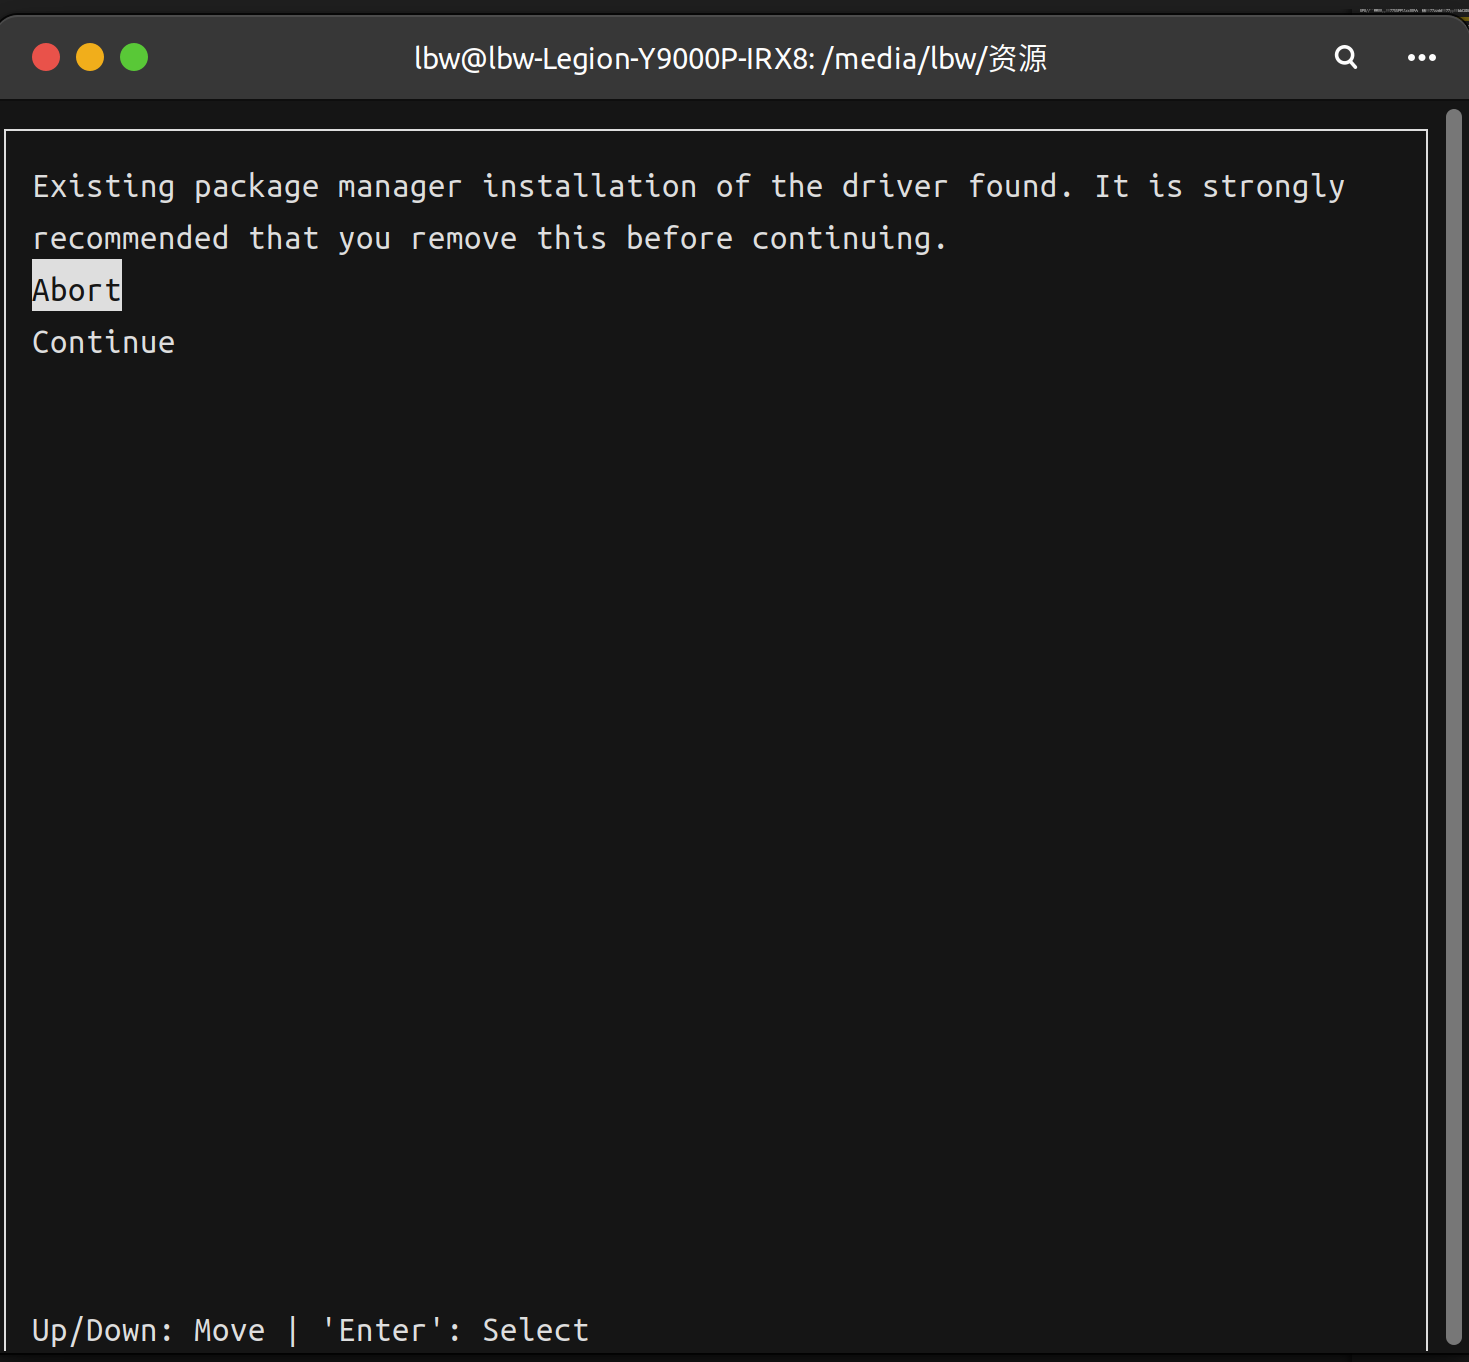
\includegraphics[width=0.7\textwidth]{CUDA_install.png}
    \caption{CUDA 安装向导}
    \label{fig:cuda_install1}
\end{figure}

选择 Continue，接受许可后进入组件选择：

\begin{figure}[H]
    \centering
    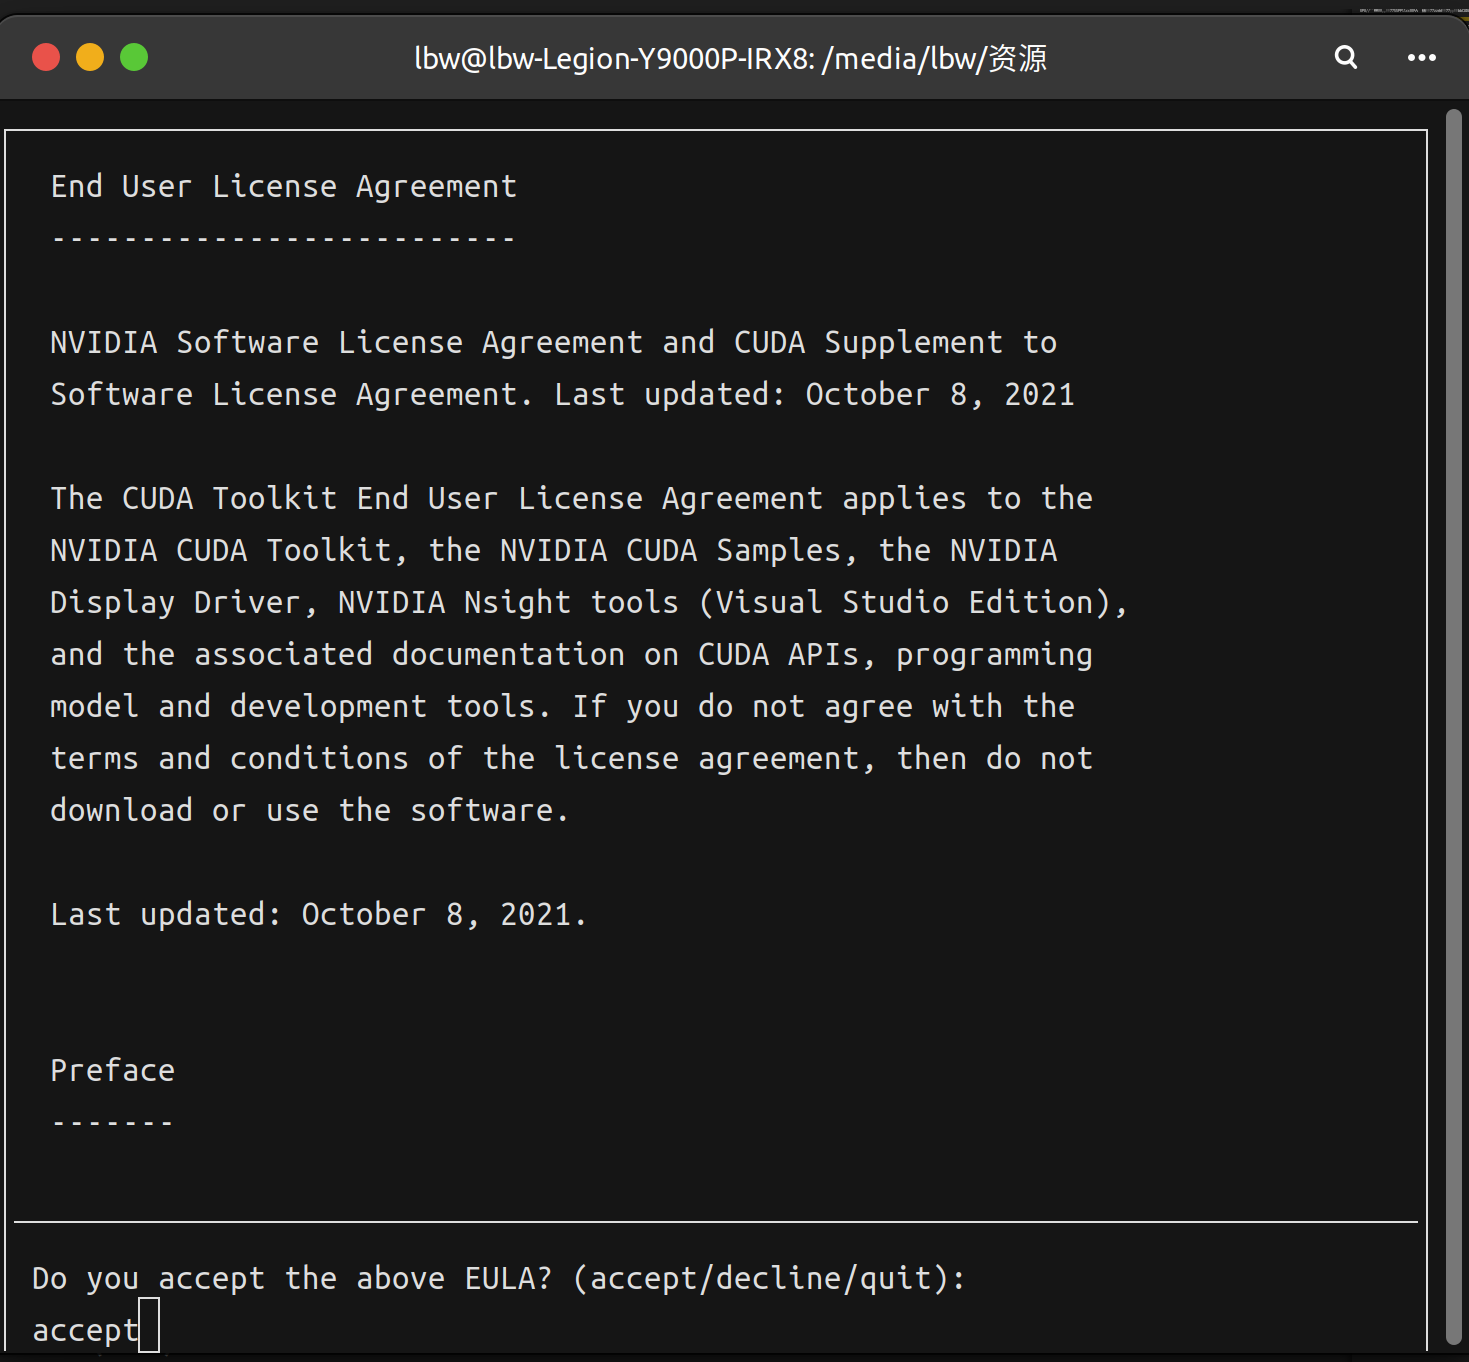
\includegraphics[width=0.7\textwidth]{CUDA_accept.png}
    \caption{接受许可}
    \label{fig:cuda_install2}
\end{figure}

\begin{figure}[H]
    \centering
    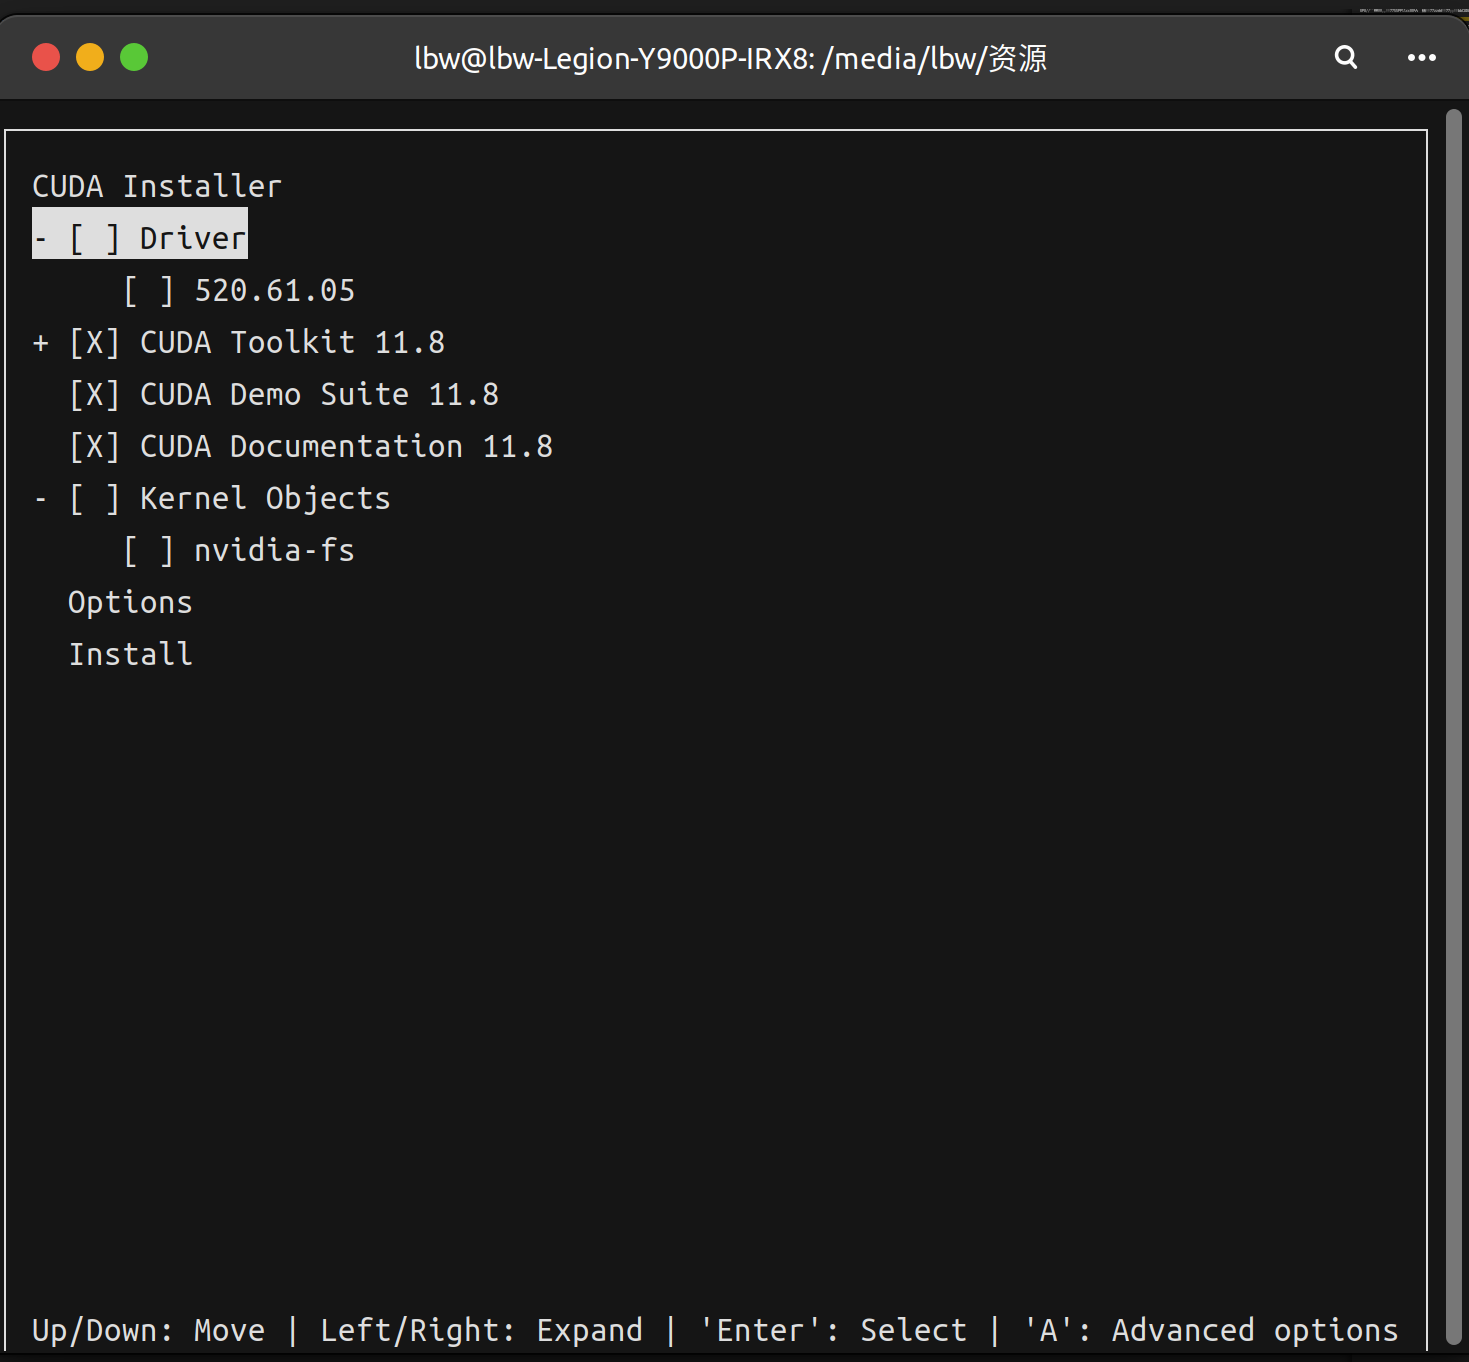
\includegraphics[width=0.7\textwidth]{CUDA_warning.png}
    \caption{组件选择：务必取消 Driver}
    \label{fig:cuda_install3}
\end{figure}

\textbf{关键：}若系统已有可用 NVIDIA 驱动，安装 Toolkit 时应用空格键\textbf{取消勾选 Driver}，只装 toolkit。
否则可能覆盖驱动导致黑屏。

按提示配置环境变量，例如：
\begin{tbash}
export PATH=/usr/local/cuda/bin:$PATH
export LD_LIBRARY_PATH=/usr/local/cuda/lib64:$LD_LIBRARY_PATH
\end{tbash}
写入 \texttt{\textasciitilde/.bashrc} 后 \texttt{source}。验证：
\begin{tbash}
nvcc --version
\end{tbash}

\begin{figure}[H]
    \centering
    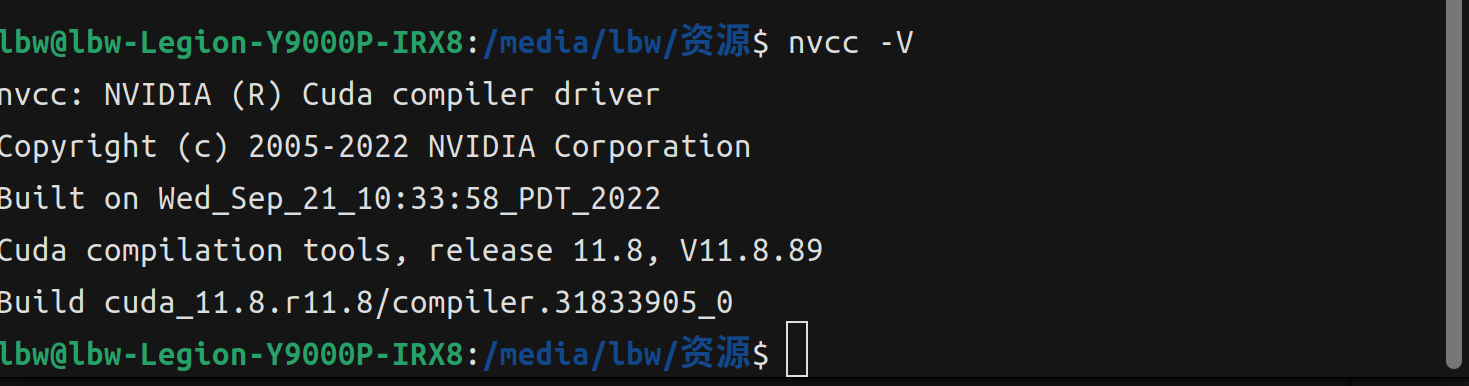
\includegraphics[width=0.7\textwidth]{CUDA_check.png}
    \caption{nvcc 版本输出示例}
    \label{fig:cuda_check}
\end{figure}

亦可用发行版包管理或 NVIDIA 官方 apt 源安装，原理相同：驱动与 toolkit 版本兼容即可。

\subsection{安装 cuDNN*}

cuDNN 是面向深度网络的加速库。需与 CUDA 主版本匹配，从 NVIDIA 开发者站点下载对应包后解压拷贝：
\begin{tbash}
tar -xzvf cudnn-*-linux-x64-*.tgz
sudo cp cuda/include/cudnn*.h /usr/local/cuda/include
sudo cp cuda/lib64/libcudnn* /usr/local/cuda/lib64
sudo chmod a+r /usr/local/cuda/include/cudnn*.h /usr/local/cuda/lib64/libcudnn*
\end{tbash}
训练框架（如带 GPU 的 PyTorch）通常自带或通过 pip/conda 拉取匹配的运行时；
手写调用 cuDNN API 时才必须显式安装开发文件。

\section{异构计算：Host 与 Device}

GPU 一般不独立运行完整操作系统任务，而是作为 CPU 的协处理器。
CPU 端称为 \textbf{host}，GPU 端称为 \textbf{device}，二者经 PCIe 等总线连接。
典型流程：
\begin{enumerate}
    \item Host 分配设备内存（\texttt{cudaMalloc}）；
    \item 将数据从 Host 拷到 Device（\texttt{cudaMemcpy}）；
    \item 启动 kernel 在 GPU 上计算；
    \item 将结果拷回 Host（\texttt{cudaMemcpy}）；
    \item 释放设备内存（\texttt{cudaFree}）。
\end{enumerate}

\begin{figure}[H]
    \centering
    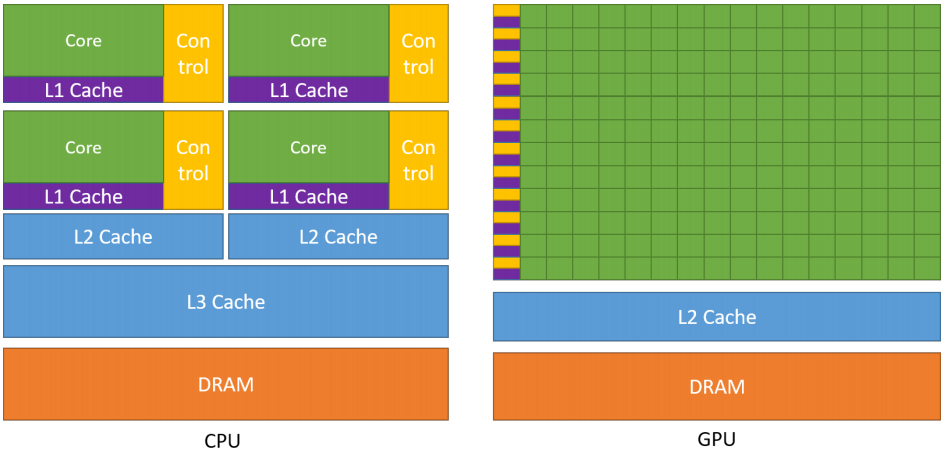
\includegraphics[width=0.85\textwidth]{Host-Device.png}
    \caption{CPU--GPU 异构架构示意}
    \label{fig:host_device}
\end{figure}

数据搬运开销不可忽视：若计算量很小而拷贝很重，整体可能比纯 CPU 更慢。
工程上应尽量减少往返拷贝，或把多步处理串在 Device 侧完成。

\section{CUDA 编程基础}

以下内容依据 NVIDIA \emph{CUDA Programming Guide} 中 Intro / Writing Kernels 章节整理。

\subsection{线程层次：Thread、Block、Grid}

Kernel 启动时创建大量线程，组织为：
\begin{itemize}
    \item \textbf{Thread}：执行同一段 kernel 代码的基本单位，通过内置变量区分各自数据；
    \item \textbf{Block}：一组可协作的线程，共享一块 \textbf{shared memory}，可用 \texttt{\_\_syncthreads()} 同步；
    \item \textbf{Grid}：若干 Block 的集合，分布在多个 SM（Streaming Multiprocessor）上执行。
\end{itemize}

核内常用内置变量：\texttt{threadIdx}、\texttt{blockIdx}、\texttt{blockDim}、\texttt{gridDim}（可达三维）。
一维全局下标常写为：
\begin{tcode}
int i = blockIdx.x * blockDim.x + threadIdx.x;
\end{tcode}

启动语法（triple chevron）：
\begin{tcode}
kernel<<<gridDim, blockDim>>>(args...);
// 或 dim3 grid(gx, gy); dim3 block(bx, by);
// kernel<<<grid, block>>>(...);
\end{tcode}
第一参数为 Grid 维度，第二参数为每个 Block 的线程数。
Block 大小常取 128、256 等，需结合占用率与问题规模调试。

\subsection{第一个例子：向量加法}

\begin{tcode}
#include <cuda_runtime.h>
#include <cstdio>

__global__ void vecAdd(const float* A, const float* B, float* C, int n) {
    int i = blockIdx.x * blockDim.x + threadIdx.x;
    if (i < n) C[i] = A[i] + B[i];
}

int main() {
    const int n = 1 << 20;
    size_t bytes = n * sizeof(float);
    float *hA = new float[n], *hB = new float[n], *hC = new float[n];
    for (int i = 0; i < n; ++i) { hA[i] = 1.f; hB[i] = 2.f; }

    float *dA, *dB, *dC;
    cudaMalloc(&dA, bytes); cudaMalloc(&dB, bytes); cudaMalloc(&dC, bytes);
    cudaMemcpy(dA, hA, bytes, cudaMemcpyHostToDevice);
    cudaMemcpy(dB, hB, bytes, cudaMemcpyHostToDevice);

    int threads = 256;
    int blocks = (n + threads - 1) / threads;
    vecAdd<<<blocks, threads>>>(dA, dB, dC, n);
    cudaDeviceSynchronize();

    cudaMemcpy(hC, dC, bytes, cudaMemcpyDeviceToHost);
    printf("C[0]=%f\n", hC[0]); // 期望 3

    cudaFree(dA); cudaFree(dB); cudaFree(dC);
    delete[] hA; delete[] hB; delete[] hC;
    return 0;
}
\end{tcode}

要点：
\begin{itemize}
    \item 设备端函数用 \texttt{\_\_global\_\_} 修饰，由 Host 启动；
    \item 必须用 \texttt{if (i < n)} 防止越界（末尾 Block 可能超出）；
    \item \texttt{cudaMemcpy} 最后一参指明方向：\texttt{HostToDevice} / \texttt{DeviceToHost} / \texttt{DeviceToDevice}。
\end{itemize}

编译示例：
\begin{tbash}
nvcc -O2 vec_add.cu -o vec_add
./vec_add
\end{tbash}

\subsection{内存层次（入门）}

\begin{itemize}
    \item \textbf{Global memory}：容量大、延迟高，\texttt{cudaMalloc} 得到的指针通常指向此处；
    \item \textbf{Shared memory}：Block 内共享的片上暂存，延迟低、容量小，适合复用数据；
    \item \textbf{Registers / Local}：每线程私有；寄存器溢出时可能落到 local memory。
\end{itemize}

Shared memory 示例骨架：
\begin{tcode}
__global__ void demo(float* out, const float* in) {
    __shared__ float tile[256];
    int tid = threadIdx.x;
    int i = blockIdx.x * blockDim.x + tid;
    tile[tid] = in[i];
    __syncthreads(); // 等待块内全部写完再读
    out[i] = tile[tid]; // 示意：实际可做归约、卷积滑窗等
}
\end{tcode}
块内协作读写前务必 \texttt{\_\_syncthreads()}，否则存在数据竞争。

\subsection{错误检查习惯}

生产代码应对每次 CUDA API 检查返回值，例如：
\begin{tcode}
#define CUDA_CHECK(call) do { \
  cudaError_t e = (call); \
  if (e != cudaSuccess) { \
    fprintf(stderr, "CUDA error %s:%d: %s\n", __FILE__, __LINE__, \
            cudaGetErrorString(e)); \
    exit(1); \
  } \
} while(0)
\end{tcode}
Kernel 启动为异步，常用 \texttt{cudaGetLastError()} 与 \texttt{cudaDeviceSynchronize()} 捕获启动/执行错误。

\subsection{与 CMake 集成}

现代 CMake（3.18+）推荐启用 CUDA 语言并链接 Toolkit 目标：
\begin{tcode}
cmake_minimum_required(VERSION 3.18)
project(cuda_demo LANGUAGES CXX CUDA)
find_package(CUDAToolkit REQUIRED)
add_executable(vec_add vec_add.cu)
target_link_libraries(vec_add PRIVATE CUDA::cudart)
\end{tcode}

\section{从算子到推理部署*}

手写 kernel 适合学习与关键热点优化；多数视觉推理优先走成熟栈：
\begin{enumerate}
    \item 训练框架导出 \textbf{ONNX}（跨框架中间表示）；
    \item 用 \textbf{TensorRT}（或 OpenVINO 等）构建优化引擎（融合算子、精度校准等）；
    \item 在线加载 \texttt{.engine} 做低延迟推理。
\end{enumerate}
TensorRT 依赖 CUDA；引擎往往与具体 GPU 架构相关，换卡常需重建。
深度学习章中的部署小节与此衔接：本卷强调 CUDA 是 GPU 路径的底座，
具体 TensorRT API 可在项目仓库与 NVIDIA 文档中深入。

\section{常见问题与边界}

\begin{itemize}
    \item 笔记本双显卡：确认进程跑在 NVIDIA 独显上（\texttt{nvidia-smi} 看进程）。
    \item WSL / 容器：需额外配置 GPU 透传，与裸机步骤不同。
    \item 无 GPU 环境：可学概念与写可在 CPU 回退的代码路径；本章验收中的运行项需有可用设备。
\end{itemize}

延伸阅读：
\url{https://docs.nvidia.com/cuda/cuda-programming-guide/02-basics/intro-to-cuda-cpp.html}。
